\documentclass[1p]{elsarticle_modified}
%\bibliographystyle{elsarticle-num}

%\usepackage[colorlinks]{hyperref}
%\usepackage{abbrmath_seonhwa} %\Abb, \Ascr, \Acal ,\Abf, \Afrak
\usepackage{amsfonts}
\usepackage{amssymb}
\usepackage{amsmath}
\usepackage{amsthm}
\usepackage{scalefnt}
\usepackage{amsbsy}
\usepackage{kotex}
\usepackage{caption}
\usepackage{subfig}
\usepackage{color}
\usepackage{graphicx}
\usepackage{xcolor} %% white, black, red, green, blue, cyan, magenta, yellow
\usepackage{float}
\usepackage{setspace}
\usepackage{hyperref}

\usepackage{tikz}
\usetikzlibrary{arrows}

\usepackage{multirow}
\usepackage{array} % fixed length table
\usepackage{hhline}

%%%%%%%%%%%%%%%%%%%%%
\makeatletter
\renewcommand*\env@matrix[1][\arraystretch]{%
	\edef\arraystretch{#1}%
	\hskip -\arraycolsep
	\let\@ifnextchar\new@ifnextchar
	\array{*\c@MaxMatrixCols c}}
\makeatother %https://tex.stackexchange.com/questions/14071/how-can-i-increase-the-line-spacing-in-a-matrix
%%%%%%%%%%%%%%%

\usepackage[normalem]{ulem}

\newcommand{\msout}[1]{\ifmmode\text{\sout{\ensuremath{#1}}}\else\sout{#1}\fi}
%SOURCE: \msout is \stkout macro in https://tex.stackexchange.com/questions/20609/strikeout-in-math-mode

\newcommand{\cancel}[1]{
	\ifmmode
	{\color{red}\msout{#1}}
	\else
	{\color{red}\sout{#1}}
	\fi
}

\newcommand{\add}[1]{
	{\color{blue}\uwave{#1}}
}

\newcommand{\replace}[2]{
	\ifmmode
	{\color{red}\msout{#1}}{\color{blue}\uwave{#2}}
	\else
	{\color{red}\sout{#1}}{\color{blue}\uwave{#2}}
	\fi
}

\newcommand{\Sol}{\mathcal{S}} %segment
\newcommand{\D}{D} %diagram
\newcommand{\A}{\mathcal{A}} %arc


%%%%%%%%%%%%%%%%%%%%%%%%%%%%%5 test

\def\sl{\operatorname{\textup{SL}}(2,\Cbb)}
\def\psl{\operatorname{\textup{PSL}}(2,\Cbb)}
\def\quan{\mkern 1mu \triangleright \mkern 1mu}

\theoremstyle{definition}
\newtheorem{thm}{Theorem}[section]
\newtheorem{prop}[thm]{Proposition}
\newtheorem{lem}[thm]{Lemma}
\newtheorem{ques}[thm]{Question}
\newtheorem{cor}[thm]{Corollary}
\newtheorem{defn}[thm]{Definition}
\newtheorem{exam}[thm]{Example}
\newtheorem{rmk}[thm]{Remark}
\newtheorem{alg}[thm]{Algorithm}

\newcommand{\I}{\sqrt{-1}}
\begin{document}

%\begin{frontmatter}
%
%\title{Boundary parabolic representations of knots up to 8 crossings}
%
%%% Group authors per affiliation:
%\author{Yunhi Cho} 
%\address{Department of Mathematics, University of Seoul, Seoul, Korea}
%\ead{yhcho@uos.ac.kr}
%
%
%\author{Seonhwa Kim} %\fnref{s_kim}}
%\address{Center for Geometry and Physics, Institute for Basic Science, Pohang, 37673, Korea}
%\ead{ryeona17@ibs.re.kr}
%
%\author{Hyuk Kim}
%\address{Department of Mathematical Sciences, Seoul National University, Seoul 08826, Korea}
%\ead{hyukkim@snu.ac.kr}
%
%\author{Seokbeom Yoon}
%\address{Department of Mathematical Sciences, Seoul National University, Seoul, 08826,  Korea}
%\ead{sbyoon15@snu.ac.kr}
%
%\begin{abstract}
%We find all boundary parabolic representation of knots up to 8 crossings.
%
%\end{abstract}
%\begin{keyword}
%    \MSC[2010] 57M25 
%\end{keyword}
%
%\end{frontmatter}

%\linenumbers
%\tableofcontents
%
\newcommand\colored[1]{\textcolor{white}{\rule[-0.35ex]{0.8em}{1.4ex}}\kern-0.8em\color{red} #1}%
%\newcommand\colored[1]{\textcolor{white}{ #1}\kern-2.17ex	\textcolor{white}{ #1}\kern-1.81ex	\textcolor{white}{ #1}\kern-2.15ex\color{red}#1	}

{\Large $\underline{11n_{89}~(K11n_{89})}$}

\setlength{\tabcolsep}{10pt}
\renewcommand{\arraystretch}{1.6}
\vspace{1cm}\begin{tabular}{m{100pt}>{\centering\arraybackslash}m{274pt}}
\multirow{5}{120pt}{
	\centering
	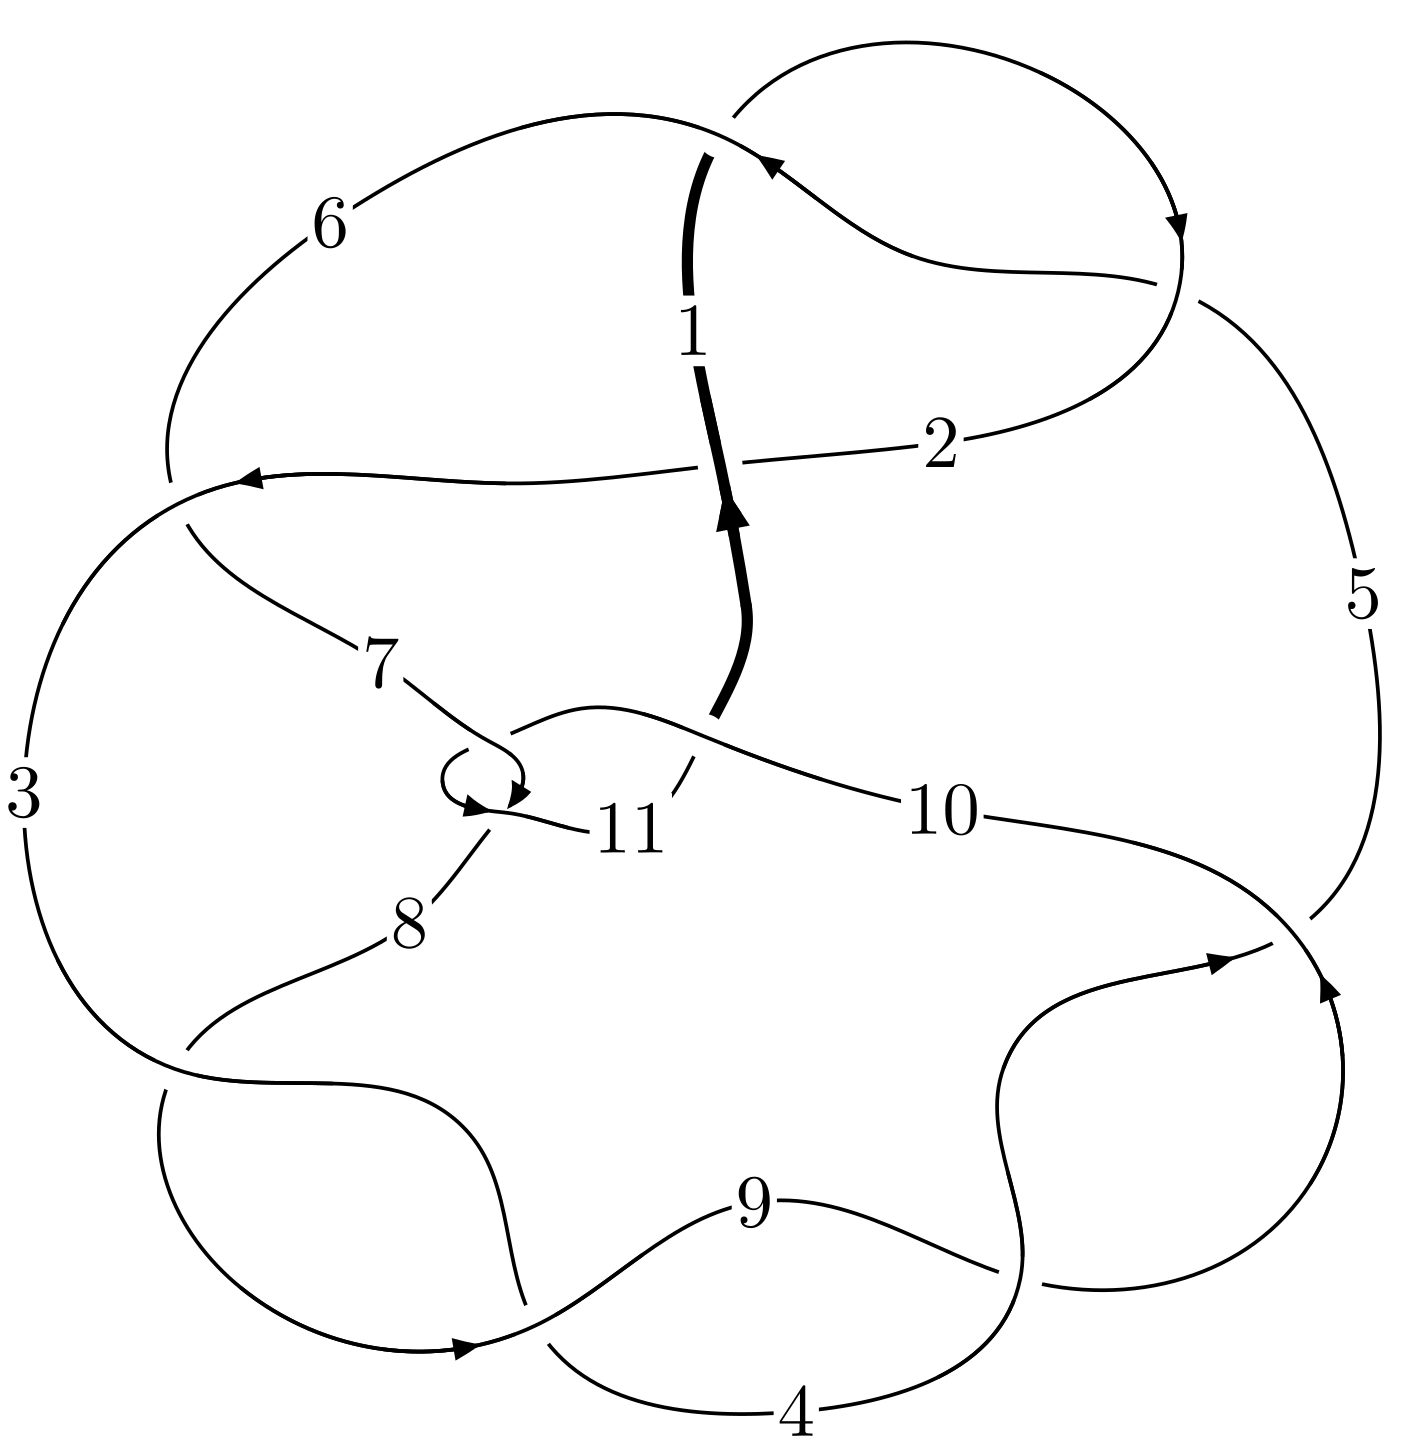
\includegraphics[width=112pt]{../../../GIT/diagram.site/Diagrams/png/705_11n_89.png}\\
\ \ \ A knot diagram\footnotemark}&
\allowdisplaybreaks
\textbf{Linearized knot diagam} \\
\cline{2-2}
 &
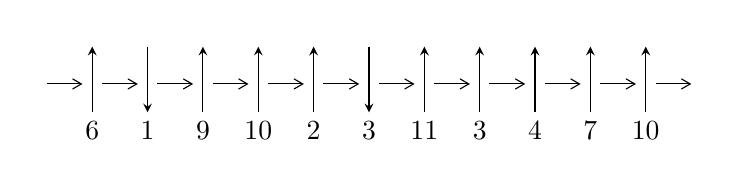
\begin{tikzpicture}[x=20pt, y=17pt]
	% nodes
	\node (C0) at (0, 0) {};
	\node (C1) at (1, 0) {};
	\node (C1U) at (1, +1) {};
	\node (C1D) at (1, -1) {6};

	\node (C2) at (2, 0) {};
	\node (C2U) at (2, +1) {};
	\node (C2D) at (2, -1) {1};

	\node (C3) at (3, 0) {};
	\node (C3U) at (3, +1) {};
	\node (C3D) at (3, -1) {9};

	\node (C4) at (4, 0) {};
	\node (C4U) at (4, +1) {};
	\node (C4D) at (4, -1) {10};

	\node (C5) at (5, 0) {};
	\node (C5U) at (5, +1) {};
	\node (C5D) at (5, -1) {2};

	\node (C6) at (6, 0) {};
	\node (C6U) at (6, +1) {};
	\node (C6D) at (6, -1) {3};

	\node (C7) at (7, 0) {};
	\node (C7U) at (7, +1) {};
	\node (C7D) at (7, -1) {11};

	\node (C8) at (8, 0) {};
	\node (C8U) at (8, +1) {};
	\node (C8D) at (8, -1) {3};

	\node (C9) at (9, 0) {};
	\node (C9U) at (9, +1) {};
	\node (C9D) at (9, -1) {4};

	\node (C10) at (10, 0) {};
	\node (C10U) at (10, +1) {};
	\node (C10D) at (10, -1) {7};

	\node (C11) at (11, 0) {};
	\node (C11U) at (11, +1) {};
	\node (C11D) at (11, -1) {10};
	\node (C12) at (12, 0) {};

	% arrows
	\draw[->,>={angle 60}]
	(C0) edge (C1) (C1) edge (C2) (C2) edge (C3) (C3) edge (C4) (C4) edge (C5) (C5) edge (C6) (C6) edge (C7) (C7) edge (C8) (C8) edge (C9) (C9) edge (C10) (C10) edge (C11) (C11) edge (C12) ;	\draw[->,>=stealth]
	(C1D) edge (C1U) (C2U) edge (C2D) (C3D) edge (C3U) (C4D) edge (C4U) (C5D) edge (C5U) (C6U) edge (C6D) (C7D) edge (C7U) (C8D) edge (C8U) (C9D) edge (C9U) (C10D) edge (C10U) (C11D) edge (C11U) ;
	\end{tikzpicture} \\
\hhline{~~} \\& 
\textbf{Solving Sequence} \\ \cline{2-2} 
 &
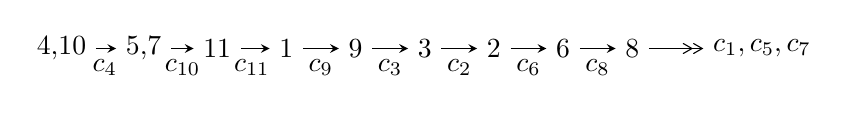
\begin{tikzpicture}[x=25pt, y=7pt]
	% node
	\node (A0) at (-1/8, 0) {4,10};
	\node (A1) at (17/16, 0) {5,7};
	\node (A2) at (17/8, 0) {11};
	\node (A3) at (25/8, 0) {1};
	\node (A4) at (33/8, 0) {9};
	\node (A5) at (41/8, 0) {3};
	\node (A6) at (49/8, 0) {2};
	\node (A7) at (57/8, 0) {6};
	\node (A8) at (65/8, 0) {8};
	\node (C1) at (1/2, -1) {$c_{4}$};
	\node (C2) at (13/8, -1) {$c_{10}$};
	\node (C3) at (21/8, -1) {$c_{11}$};
	\node (C4) at (29/8, -1) {$c_{9}$};
	\node (C5) at (37/8, -1) {$c_{3}$};
	\node (C6) at (45/8, -1) {$c_{2}$};
	\node (C7) at (53/8, -1) {$c_{6}$};
	\node (C8) at (61/8, -1) {$c_{8}$};
	\node (A9) at (10, 0) {$c_{1},c_{5},c_{7}$};

	% edge
	\draw[->,>=stealth]	
	(A0) edge (A1) (A1) edge (A2) (A2) edge (A3) (A3) edge (A4) (A4) edge (A5) (A5) edge (A6) (A6) edge (A7) (A7) edge (A8) ;
	\draw[->>,>={angle 60}]	
	(A8) edge (A9);
\end{tikzpicture} \\ 

\end{tabular} \\

\footnotetext{
The image of knot diagram is generated by the software ``\textbf{Draw programme}" developed by Andrew Bartholomew(\url{http://www.layer8.co.uk/maths/draw/index.htm\#Running-draw}), where we modified some parts for our purpose(\url{https://github.com/CATsTAILs/LinksPainter}).
}\phantom \\ \newline 
\centering \textbf{Ideals for irreducible components\footnotemark of $X_{\text{par}}$} 
 
\begin{align*}
I^u_{1}&=\langle 
1.81408\times10^{16} u^{35}+4.53180\times10^{15} u^{34}+\cdots+1.44921\times10^{16} b+6.92452\times10^{16},\\
\phantom{I^u_{1}}&\phantom{= \langle  }-7.36698\times10^{15} u^{35}-2.71053\times10^{15} u^{34}+\cdots+1.44921\times10^{16} a-3.17098\times10^{16},\;u^{36}- u^{35}+\cdots+12 u-4\rangle \\
I^u_{2}&=\langle 
b^2+2 b u- b- u+3,\;2 a- u,\;u^2-2\rangle \\
\\
I^v_{1}&=\langle 
a,\;b+v-1,\;v^2- v+1\rangle \\
\end{align*}
\raggedright * 3 irreducible components of $\dim_{\mathbb{C}}=0$, with total 42 representations.\\
\footnotetext{All coefficients of polynomials are rational numbers. But the coefficients are sometimes approximated in decimal forms when there is not enough margin.}
\newpage
\renewcommand{\arraystretch}{1}
\centering \section*{I. $I^u_{1}= \langle 1.81\times10^{16} u^{35}+4.53\times10^{15} u^{34}+\cdots+1.45\times10^{16} b+6.92\times10^{16},\;-7.37\times10^{15} u^{35}-2.71\times10^{15} u^{34}+\cdots+1.45\times10^{16} a-3.17\times10^{16},\;u^{36}- u^{35}+\cdots+12 u-4 \rangle$}
\flushleft \textbf{(i) Arc colorings}\\
\begin{tabular}{m{7pt} m{180pt} m{7pt} m{180pt} }
\flushright $a_{4}=$&$\begin{pmatrix}1\\0\end{pmatrix}$ \\
\flushright $a_{10}=$&$\begin{pmatrix}0\\u\end{pmatrix}$ \\
\flushright $a_{5}=$&$\begin{pmatrix}1\\- u^2\end{pmatrix}$ \\
\flushright $a_{7}=$&$\begin{pmatrix}0.508345 u^{35}+0.187035 u^{34}+\cdots-3.81933 u+2.18808\\-1.25177 u^{35}-0.312708 u^{34}+\cdots+10.6982 u-4.77814\end{pmatrix}$ \\
\flushright $a_{11}=$&$\begin{pmatrix}0.995471 u^{35}+0.0679041 u^{34}+\cdots-10.1216 u+3.89180\\-0.252045 u^{35}+0.0577695 u^{34}+\cdots+3.24270 u-1.30174\end{pmatrix}$ \\
\flushright $a_{1}=$&$\begin{pmatrix}0.995471 u^{35}+0.0679041 u^{34}+\cdots-10.1216 u+3.89180\\-1.49385 u^{35}-0.192804 u^{34}+\cdots+12.0213 u-5.55524\end{pmatrix}$ \\
\flushright $a_{9}=$&$\begin{pmatrix}- u\\u\end{pmatrix}$ \\
\flushright $a_{3}=$&$\begin{pmatrix}- u^2+1\\u^2\end{pmatrix}$ \\
\flushright $a_{2}=$&$\begin{pmatrix}1.29114 u^{35}+0.157626 u^{34}+\cdots-12.6782 u+5.68748\\-1.28270 u^{35}-0.365443 u^{34}+\cdots+10.3098 u-3.90050\end{pmatrix}$ \\
\flushright $a_{6}=$&$\begin{pmatrix}0.498382 u^{35}+0.124900 u^{34}+\cdots-1.89976 u+1.66344\\-1.49385 u^{35}-0.192804 u^{34}+\cdots+12.0213 u-5.55524\end{pmatrix}$ \\
\flushright $a_{8}=$&$\begin{pmatrix}u^3-2 u\\- u^3+u\end{pmatrix}$\\ \flushright $a_{8}=$&$\begin{pmatrix}u^3-2 u\\- u^3+u\end{pmatrix}$\\&\end{tabular}
\flushleft \textbf{(ii) Obstruction class $= -1$}\\~\\
\flushleft \textbf{(iii) Cusp Shapes $= -\frac{2185176855038490}{3623024810197363} u^{35}-\frac{2137823921618481}{3623024810197363} u^{34}+\cdots-\frac{32140848155027584}{3623024810197363} u+\frac{31012404119150980}{3623024810197363}$}\\~\\
\newpage\renewcommand{\arraystretch}{1}
\flushleft \textbf{(iv) u-Polynomials at the component}\newline \\
\begin{tabular}{m{50pt}|m{274pt}}
Crossings & \hspace{64pt}u-Polynomials at each crossing \\
\hline $$\begin{aligned}c_{1},c_{5}\end{aligned}$$&$\begin{aligned}
&u^{36}-2 u^{35}+\cdots-6 u+1
\end{aligned}$\\
\hline $$\begin{aligned}c_{2}\end{aligned}$$&$\begin{aligned}
&u^{36}+20 u^{35}+\cdots-6 u+1
\end{aligned}$\\
\hline $$\begin{aligned}c_{3},c_{4},c_{8}\\c_{9}\end{aligned}$$&$\begin{aligned}
&u^{36}- u^{35}+\cdots+12 u-4
\end{aligned}$\\
\hline $$\begin{aligned}c_{6}\end{aligned}$$&$\begin{aligned}
&u^{36}+2 u^{35}+\cdots+6 u+13
\end{aligned}$\\
\hline $$\begin{aligned}c_{7},c_{10}\end{aligned}$$&$\begin{aligned}
&u^{36}-3 u^{35}+\cdots+13 u-7
\end{aligned}$\\
\hline $$\begin{aligned}c_{11}\end{aligned}$$&$\begin{aligned}
&u^{36}-13 u^{35}+\cdots-687 u+49
\end{aligned}$\\
\hline
\end{tabular}\\~\\
\newpage\renewcommand{\arraystretch}{1}
\flushleft \textbf{(v) Riley Polynomials at the component}\newline \\
\begin{tabular}{m{50pt}|m{274pt}}
Crossings & \hspace{64pt}Riley Polynomials at each crossing \\
\hline $$\begin{aligned}c_{1},c_{5}\end{aligned}$$&$\begin{aligned}
&y^{36}+20 y^{35}+\cdots-6 y+1
\end{aligned}$\\
\hline $$\begin{aligned}c_{2}\end{aligned}$$&$\begin{aligned}
&y^{36}-4 y^{35}+\cdots-142 y+1
\end{aligned}$\\
\hline $$\begin{aligned}c_{3},c_{4},c_{8}\\c_{9}\end{aligned}$$&$\begin{aligned}
&y^{36}-31 y^{35}+\cdots+80 y+16
\end{aligned}$\\
\hline $$\begin{aligned}c_{6}\end{aligned}$$&$\begin{aligned}
&y^{36}-28 y^{35}+\cdots-3962 y+169
\end{aligned}$\\
\hline $$\begin{aligned}c_{7},c_{10}\end{aligned}$$&$\begin{aligned}
&y^{36}-13 y^{35}+\cdots-687 y+49
\end{aligned}$\\
\hline $$\begin{aligned}c_{11}\end{aligned}$$&$\begin{aligned}
&y^{36}+27 y^{35}+\cdots-44983 y+2401
\end{aligned}$\\
\hline
\end{tabular}\\~\\
\newpage\flushleft \textbf{(vi) Complex Volumes and Cusp Shapes}
$$\begin{array}{c|c|c}  
\text{Solutions to }I^u_{1}& \I (\text{vol} + \sqrt{-1}CS) & \text{Cusp shape}\\
 \hline 
\begin{aligned}
u &= -0.194833 + 0.923873 I \\
a &= -1.10823 - 0.89470 I \\
b &= \phantom{-}1.34994 + 0.54291 I\end{aligned}
 & -6.59180 - 8.00171 I & \phantom{-}4.29537 + 5.98015 I \\ \hline\begin{aligned}
u &= -0.194833 - 0.923873 I \\
a &= -1.10823 + 0.89470 I \\
b &= \phantom{-}1.34994 - 0.54291 I\end{aligned}
 & -6.59180 + 8.00171 I & \phantom{-}4.29537 - 5.98015 I \\ \hline\begin{aligned}
u &= \phantom{-}0.006560 + 0.931824 I \\
a &= -1.025890 - 0.856109 I \\
b &= \phantom{-}1.239880 + 0.450718 I\end{aligned}
 & -7.38383 + 1.35991 I & \phantom{-}2.81294 - 0.73046 I \\ \hline\begin{aligned}
u &= \phantom{-}0.006560 - 0.931824 I \\
a &= -1.025890 + 0.856109 I \\
b &= \phantom{-}1.239880 - 0.450718 I\end{aligned}
 & -7.38383 - 1.35991 I & \phantom{-}2.81294 + 0.73046 I \\ \hline\begin{aligned}
u &= \phantom{-}0.109745 + 0.850278 I \\
a &= \phantom{-}1.058100 - 0.923490 I \\
b &= -1.266800 + 0.563919 I\end{aligned}
 & -3.22625 + 3.00094 I & \phantom{-}6.75961 - 2.89336 I \\ \hline\begin{aligned}
u &= \phantom{-}0.109745 - 0.850278 I \\
a &= \phantom{-}1.058100 + 0.923490 I \\
b &= -1.266800 - 0.563919 I\end{aligned}
 & -3.22625 - 3.00094 I & \phantom{-}6.75961 + 2.89336 I \\ \hline\begin{aligned}
u &= \phantom{-}1.160570 + 0.158096 I \\
a &= \phantom{-}1.122800 - 0.199847 I \\
b &= -1.61805 + 0.12059 I\end{aligned}
 & \phantom{-}3.84173 + 3.51209 I & \phantom{-}9.42797 - 4.38206 I \\ \hline\begin{aligned}
u &= \phantom{-}1.160570 - 0.158096 I \\
a &= \phantom{-}1.122800 + 0.199847 I \\
b &= -1.61805 - 0.12059 I\end{aligned}
 & \phantom{-}3.84173 - 3.51209 I & \phantom{-}9.42797 + 4.38206 I \\ \hline\begin{aligned}
u &= -1.077610 + 0.525072 I \\
a &= \phantom{-}0.298720 + 0.977705 I \\
b &= \phantom{-}0.481253 + 0.080718 I\end{aligned}
 & -3.88454 + 2.88072 I & \phantom{-}5.75517 - 2.19113 I \\ \hline\begin{aligned}
u &= -1.077610 - 0.525072 I \\
a &= \phantom{-}0.298720 - 0.977705 I \\
b &= \phantom{-}0.481253 - 0.080718 I\end{aligned}
 & -3.88454 - 2.88072 I & \phantom{-}5.75517 + 2.19113 I\\
 \hline 
 \end{array}$$\newpage$$\begin{array}{c|c|c}  
\text{Solutions to }I^u_{1}& \I (\text{vol} + \sqrt{-1}CS) & \text{Cusp shape}\\
 \hline 
\begin{aligned}
u &= \phantom{-}1.202650 + 0.097073 I \\
a &= -0.646364 - 0.353578 I \\
b &= -0.21399 - 1.65792 I\end{aligned}
 & \phantom{-}4.33907 - 0.62358 I & \phantom{-}10.41420 - 0.63892 I \\ \hline\begin{aligned}
u &= \phantom{-}1.202650 - 0.097073 I \\
a &= -0.646364 + 0.353578 I \\
b &= -0.21399 + 1.65792 I\end{aligned}
 & \phantom{-}4.33907 + 0.62358 I & \phantom{-}10.41420 + 0.63892 I \\ \hline\begin{aligned}
u &= \phantom{-}1.182650 + 0.387668 I \\
a &= -0.269222 + 0.813754 I \\
b &= -0.610573 + 0.189166 I\end{aligned}
 & \phantom{-}0.05037 + 1.45720 I & \phantom{-}9.46667 - 0.65893 I \\ \hline\begin{aligned}
u &= \phantom{-}1.182650 - 0.387668 I \\
a &= -0.269222 - 0.813754 I \\
b &= -0.610573 - 0.189166 I\end{aligned}
 & \phantom{-}0.05037 - 1.45720 I & \phantom{-}9.46667 + 0.65893 I \\ \hline\begin{aligned}
u &= -1.236460 + 0.192085 I \\
a &= \phantom{-}0.735931 - 0.323447 I \\
b &= -0.46964 - 1.88597 I\end{aligned}
 & \phantom{-}4.64327 - 4.73682 I & \phantom{-}11.38513 + 6.59168 I \\ \hline\begin{aligned}
u &= -1.236460 - 0.192085 I \\
a &= \phantom{-}0.735931 + 0.323447 I \\
b &= -0.46964 + 1.88597 I\end{aligned}
 & \phantom{-}4.64327 + 4.73682 I & \phantom{-}11.38513 - 6.59168 I \\ \hline\begin{aligned}
u &= -0.577288 + 0.463180 I \\
a &= \phantom{-}0.811817 - 0.556107 I \\
b &= -0.692193 - 0.136688 I\end{aligned}
 & -2.03068 - 1.81473 I & \phantom{-}2.83557 + 4.64572 I \\ \hline\begin{aligned}
u &= -0.577288 - 0.463180 I \\
a &= \phantom{-}0.811817 + 0.556107 I \\
b &= -0.692193 + 0.136688 I\end{aligned}
 & -2.03068 + 1.81473 I & \phantom{-}2.83557 - 4.64572 I \\ \hline\begin{aligned}
u &= -1.31774\phantom{ +0.000000I} \\
a &= -0.894179\phantom{ +0.000000I} \\
b &= \phantom{-}1.49912\phantom{ +0.000000I}\end{aligned}
 & \phantom{-}6.40417\phantom{ +0.000000I} & \phantom{-}14.3790\phantom{ +0.000000I} \\ \hline\begin{aligned}
u &= \phantom{-}1.280170 + 0.461183 I \\
a &= -0.895029 - 0.349023 I \\
b &= \phantom{-}1.40509 - 1.14928 I\end{aligned}
 & -3.43518 + 3.60339 I & \phantom{-}6.07450 - 2.50762 I\\
 \hline 
 \end{array}$$\newpage$$\begin{array}{c|c|c}  
\text{Solutions to }I^u_{1}& \I (\text{vol} + \sqrt{-1}CS) & \text{Cusp shape}\\
 \hline 
\begin{aligned}
u &= \phantom{-}1.280170 - 0.461183 I \\
a &= -0.895029 + 0.349023 I \\
b &= \phantom{-}1.40509 + 1.14928 I\end{aligned}
 & -3.43518 - 3.60339 I & \phantom{-}6.07450 + 2.50762 I \\ \hline\begin{aligned}
u &= -1.290060 + 0.452109 I \\
a &= \phantom{-}0.147894 + 0.839120 I \\
b &= \phantom{-}0.685533 + 0.078345 I\end{aligned}
 & -3.35690 - 6.29314 I & \phantom{-}6.15059 + 3.94061 I \\ \hline\begin{aligned}
u &= -1.290060 - 0.452109 I \\
a &= \phantom{-}0.147894 - 0.839120 I \\
b &= \phantom{-}0.685533 - 0.078345 I\end{aligned}
 & -3.35690 + 6.29314 I & \phantom{-}6.15059 - 3.94061 I \\ \hline\begin{aligned}
u &= -1.355620 + 0.380756 I \\
a &= \phantom{-}0.878387 - 0.297489 I \\
b &= -1.57977 - 1.46639 I\end{aligned}
 & \phantom{-}1.38910 - 7.43800 I & \phantom{-}11.20734 + 4.77385 I \\ \hline\begin{aligned}
u &= -1.355620 - 0.380756 I \\
a &= \phantom{-}0.878387 + 0.297489 I \\
b &= -1.57977 + 1.46639 I\end{aligned}
 & \phantom{-}1.38910 + 7.43800 I & \phantom{-}11.20734 - 4.77385 I \\ \hline\begin{aligned}
u &= -1.43819 + 0.07165 I \\
a &= -0.701955 - 0.180604 I \\
b &= \phantom{-}1.401880 + 0.072692 I\end{aligned}
 & \phantom{-}6.55786 - 0.26724 I & \phantom{-}12.41884 - 1.59842 I \\ \hline\begin{aligned}
u &= -1.43819 - 0.07165 I \\
a &= -0.701955 + 0.180604 I \\
b &= \phantom{-}1.401880 - 0.072692 I\end{aligned}
 & \phantom{-}6.55786 + 0.26724 I & \phantom{-}12.41884 + 1.59842 I \\ \hline\begin{aligned}
u &= \phantom{-}1.41123 + 0.40473 I \\
a &= -0.905027 - 0.281003 I \\
b &= \phantom{-}1.79130 - 1.37903 I\end{aligned}
 & -1.51226 + 12.78080 I & \phantom{-}7.00000 - 7.80857 I \\ \hline\begin{aligned}
u &= \phantom{-}1.41123 - 0.40473 I \\
a &= -0.905027 + 0.281003 I \\
b &= \phantom{-}1.79130 + 1.37903 I\end{aligned}
 & -1.51226 - 12.78080 I & \phantom{-}7.00000 + 7.80857 I \\ \hline\begin{aligned}
u &= \phantom{-}1.50740 + 0.00063 I \\
a &= \phantom{-}0.404596 + 0.237890 I \\
b &= -1.296770 - 0.039394 I\end{aligned}
 & \phantom{-}5.02009 + 2.85591 I & \phantom{-}7.00000 - 5.56949 I\\
 \hline 
 \end{array}$$\newpage$$\begin{array}{c|c|c}  
\text{Solutions to }I^u_{1}& \I (\text{vol} + \sqrt{-1}CS) & \text{Cusp shape}\\
 \hline 
\begin{aligned}
u &= \phantom{-}1.50740 - 0.00063 I \\
a &= \phantom{-}0.404596 - 0.237890 I \\
b &= -1.296770 + 0.039394 I\end{aligned}
 & \phantom{-}5.02009 - 2.85591 I & \phantom{-}7.00000 + 5.56949 I \\ \hline\begin{aligned}
u &= \phantom{-}0.226004 + 0.427139 I \\
a &= -0.81515 + 2.22304 I \\
b &= -0.0399825 - 0.0159679 I\end{aligned}
 & \phantom{-}1.14397 - 1.32004 I & \phantom{-}4.86119 - 2.11551 I \\ \hline\begin{aligned}
u &= \phantom{-}0.226004 - 0.427139 I \\
a &= -0.81515 - 2.22304 I \\
b &= -0.0399825 + 0.0159679 I\end{aligned}
 & \phantom{-}1.14397 + 1.32004 I & \phantom{-}4.86119 + 2.11551 I \\ \hline\begin{aligned}
u &= \phantom{-}0.452153\phantom{ +0.000000I} \\
a &= -1.04552\phantom{ +0.000000I} \\
b &= \phantom{-}0.187974\phantom{ +0.000000I}\end{aligned}
 & \phantom{-}0.718633\phantom{ +0.000000I} & \phantom{-}13.9020\phantom{ +0.000000I} \\ \hline\begin{aligned}
u &= \phantom{-}0.015889 + 0.435860 I \\
a &= \phantom{-}0.37848 - 1.46882 I \\
b &= -0.410669 + 1.206820 I\end{aligned}
 & \phantom{-}0.87457 + 2.36441 I & \phantom{-}2.54968 - 4.98912 I \\ \hline\begin{aligned}
u &= \phantom{-}0.015889 - 0.435860 I \\
a &= \phantom{-}0.37848 + 1.46882 I \\
b &= -0.410669 - 1.206820 I\end{aligned}
 & \phantom{-}0.87457 - 2.36441 I & \phantom{-}2.54968 + 4.98912 I\\
 \hline 
 \end{array}$$\newpage\newpage\renewcommand{\arraystretch}{1}
\centering \section*{II. $I^u_{2}= \langle b^2+2 b u- b- u+3,\;2 a- u,\;u^2-2 \rangle$}
\flushleft \textbf{(i) Arc colorings}\\
\begin{tabular}{m{7pt} m{180pt} m{7pt} m{180pt} }
\flushright $a_{4}=$&$\begin{pmatrix}1\\0\end{pmatrix}$ \\
\flushright $a_{10}=$&$\begin{pmatrix}0\\u\end{pmatrix}$ \\
\flushright $a_{5}=$&$\begin{pmatrix}1\\-2\end{pmatrix}$ \\
\flushright $a_{7}=$&$\begin{pmatrix}\frac{1}{2} u\\b\end{pmatrix}$ \\
\flushright $a_{11}=$&$\begin{pmatrix}\frac{1}{2} u\\b+u\end{pmatrix}$ \\
\flushright $a_{1}=$&$\begin{pmatrix}\frac{1}{2} u\\b\end{pmatrix}$ \\
\flushright $a_{9}=$&$\begin{pmatrix}- u\\u\end{pmatrix}$ \\
\flushright $a_{3}=$&$\begin{pmatrix}-1\\2\end{pmatrix}$ \\
\flushright $a_{2}=$&$\begin{pmatrix}\frac{1}{2} b u\\- b u+b+u-1\end{pmatrix}$ \\
\flushright $a_{6}=$&$\begin{pmatrix}b+\frac{3}{2} u\\- b-2 u\end{pmatrix}$ \\
\flushright $a_{8}=$&$\begin{pmatrix}0\\- u\end{pmatrix}$\\ \flushright $a_{8}=$&$\begin{pmatrix}0\\- u\end{pmatrix}$\\&\end{tabular}
\flushleft \textbf{(ii) Obstruction class $= 1$}\\~\\
\flushleft \textbf{(iii) Cusp Shapes $= 4 b+4 u+12$}\\~\\
\newpage\renewcommand{\arraystretch}{1}
\flushleft \textbf{(iv) u-Polynomials at the component}\newline \\
\begin{tabular}{m{50pt}|m{274pt}}
Crossings & \hspace{64pt}u-Polynomials at each crossing \\
\hline $$\begin{aligned}c_{1},c_{6}\end{aligned}$$&$\begin{aligned}
&(u^2- u+1)^2
\end{aligned}$\\
\hline $$\begin{aligned}c_{2},c_{5}\end{aligned}$$&$\begin{aligned}
&(u^2+u+1)^2
\end{aligned}$\\
\hline $$\begin{aligned}c_{3},c_{4},c_{8}\\c_{9}\end{aligned}$$&$\begin{aligned}
&(u^2-2)^2
\end{aligned}$\\
\hline $$\begin{aligned}c_{7},c_{11}\end{aligned}$$&$\begin{aligned}
&(u-1)^4
\end{aligned}$\\
\hline $$\begin{aligned}c_{10}\end{aligned}$$&$\begin{aligned}
&(u+1)^4
\end{aligned}$\\
\hline
\end{tabular}\\~\\
\newpage\renewcommand{\arraystretch}{1}
\flushleft \textbf{(v) Riley Polynomials at the component}\newline \\
\begin{tabular}{m{50pt}|m{274pt}}
Crossings & \hspace{64pt}Riley Polynomials at each crossing \\
\hline $$\begin{aligned}c_{1},c_{2},c_{5}\\c_{6}\end{aligned}$$&$\begin{aligned}
&(y^2+y+1)^2
\end{aligned}$\\
\hline $$\begin{aligned}c_{3},c_{4},c_{8}\\c_{9}\end{aligned}$$&$\begin{aligned}
&(y-2)^4
\end{aligned}$\\
\hline $$\begin{aligned}c_{7},c_{10},c_{11}\end{aligned}$$&$\begin{aligned}
&(y-1)^4
\end{aligned}$\\
\hline
\end{tabular}\\~\\
\newpage\flushleft \textbf{(vi) Complex Volumes and Cusp Shapes}
$$\begin{array}{c|c|c}  
\text{Solutions to }I^u_{2}& \I (\text{vol} + \sqrt{-1}CS) & \text{Cusp shape}\\
 \hline 
\begin{aligned}
u &= \phantom{-}1.41421\phantom{ +0.000000I} \\
a &= \phantom{-}0.707107\phantom{ +0.000000I} \\
b &= -0.914214 + 0.866025 I\end{aligned}
 & \phantom{-}6.57974 - 2.02988 I & \phantom{-}14.0000 + 3.4641 I \\ \hline\begin{aligned}
u &= \phantom{-}1.41421\phantom{ +0.000000I} \\
a &= \phantom{-}0.707107\phantom{ +0.000000I} \\
b &= -0.914214 - 0.866025 I\end{aligned}
 & \phantom{-}6.57974 + 2.02988 I & \phantom{-}14.0000 - 3.4641 I \\ \hline\begin{aligned}
u &= -1.41421\phantom{ +0.000000I} \\
a &= -0.707107\phantom{ +0.000000I} \\
b &= \phantom{-}1.91421 + 0.86603 I\end{aligned}
 & \phantom{-}6.57974 - 2.02988 I & \phantom{-}14.0000 + 3.4641 I \\ \hline\begin{aligned}
u &= -1.41421\phantom{ +0.000000I} \\
a &= -0.707107\phantom{ +0.000000I} \\
b &= \phantom{-}1.91421 - 0.86603 I\end{aligned}
 & \phantom{-}6.57974 + 2.02988 I & \phantom{-}14.0000 - 3.4641 I\\
 \hline 
 \end{array}$$\newpage\newpage\renewcommand{\arraystretch}{1}
\centering \section*{III. $I^v_{1}= \langle a,\;b+v-1,\;v^2- v+1 \rangle$}
\flushleft \textbf{(i) Arc colorings}\\
\begin{tabular}{m{7pt} m{180pt} m{7pt} m{180pt} }
\flushright $a_{4}=$&$\begin{pmatrix}1\\0\end{pmatrix}$ \\
\flushright $a_{10}=$&$\begin{pmatrix}v\\0\end{pmatrix}$ \\
\flushright $a_{5}=$&$\begin{pmatrix}1\\0\end{pmatrix}$ \\
\flushright $a_{7}=$&$\begin{pmatrix}0\\- v+1\end{pmatrix}$ \\
\flushright $a_{11}=$&$\begin{pmatrix}v\\v-1\end{pmatrix}$ \\
\flushright $a_{1}=$&$\begin{pmatrix}0\\v-1\end{pmatrix}$ \\
\flushright $a_{9}=$&$\begin{pmatrix}v\\0\end{pmatrix}$ \\
\flushright $a_{3}=$&$\begin{pmatrix}1\\0\end{pmatrix}$ \\
\flushright $a_{2}=$&$\begin{pmatrix}1\\v\end{pmatrix}$ \\
\flushright $a_{6}=$&$\begin{pmatrix}- v+1\\- v+1\end{pmatrix}$ \\
\flushright $a_{8}=$&$\begin{pmatrix}v\\0\end{pmatrix}$\\ \flushright $a_{8}=$&$\begin{pmatrix}v\\0\end{pmatrix}$\\&\end{tabular}
\flushleft \textbf{(ii) Obstruction class $= 1$}\\~\\
\flushleft \textbf{(iii) Cusp Shapes $= -4 v+14$}\\~\\
\newpage\renewcommand{\arraystretch}{1}
\flushleft \textbf{(iv) u-Polynomials at the component}\newline \\
\begin{tabular}{m{50pt}|m{274pt}}
Crossings & \hspace{64pt}u-Polynomials at each crossing \\
\hline $$\begin{aligned}c_{1},c_{2},c_{6}\end{aligned}$$&$\begin{aligned}
&u^2+u+1
\end{aligned}$\\
\hline $$\begin{aligned}c_{3},c_{4},c_{8}\\c_{9}\end{aligned}$$&$\begin{aligned}
&u^2
\end{aligned}$\\
\hline $$\begin{aligned}c_{5}\end{aligned}$$&$\begin{aligned}
&u^2- u+1
\end{aligned}$\\
\hline $$\begin{aligned}c_{7}\end{aligned}$$&$\begin{aligned}
&(u+1)^2
\end{aligned}$\\
\hline $$\begin{aligned}c_{10},c_{11}\end{aligned}$$&$\begin{aligned}
&(u-1)^2
\end{aligned}$\\
\hline
\end{tabular}\\~\\
\newpage\renewcommand{\arraystretch}{1}
\flushleft \textbf{(v) Riley Polynomials at the component}\newline \\
\begin{tabular}{m{50pt}|m{274pt}}
Crossings & \hspace{64pt}Riley Polynomials at each crossing \\
\hline $$\begin{aligned}c_{1},c_{2},c_{5}\\c_{6}\end{aligned}$$&$\begin{aligned}
&y^2+y+1
\end{aligned}$\\
\hline $$\begin{aligned}c_{3},c_{4},c_{8}\\c_{9}\end{aligned}$$&$\begin{aligned}
&y^2
\end{aligned}$\\
\hline $$\begin{aligned}c_{7},c_{10},c_{11}\end{aligned}$$&$\begin{aligned}
&(y-1)^2
\end{aligned}$\\
\hline
\end{tabular}\\~\\
\newpage\flushleft \textbf{(vi) Complex Volumes and Cusp Shapes}
$$\begin{array}{c|c|c}  
\text{Solutions to }I^v_{1}& \I (\text{vol} + \sqrt{-1}CS) & \text{Cusp shape}\\
 \hline 
\begin{aligned}
v &= \phantom{-}0.500000 + 0.866025 I \\
a &= \phantom{-0.000000 } 0 \\
b &= \phantom{-}0.500000 - 0.866025 I\end{aligned}
 & \phantom{-}1.64493 + 2.02988 I & \phantom{-}12.00000 - 3.46410 I \\ \hline\begin{aligned}
v &= \phantom{-}0.500000 - 0.866025 I \\
a &= \phantom{-0.000000 } 0 \\
b &= \phantom{-}0.500000 + 0.866025 I\end{aligned}
 & \phantom{-}1.64493 - 2.02988 I & \phantom{-}12.00000 + 3.46410 I\\
 \hline 
 \end{array}$$\newpage
\newpage\renewcommand{\arraystretch}{1}
\centering \section*{ IV. u-Polynomials}
\begin{tabular}{m{50pt}|m{274pt}}
Crossings & \hspace{64pt}u-Polynomials at each crossing \\
\hline $$\begin{aligned}c_{1}\end{aligned}$$&$\begin{aligned}
&((u^2- u+1)^2)(u^2+u+1)(u^{36}-2 u^{35}+\cdots-6 u+1)
\end{aligned}$\\
\hline $$\begin{aligned}c_{2}\end{aligned}$$&$\begin{aligned}
&((u^2+u+1)^3)(u^{36}+20 u^{35}+\cdots-6 u+1)
\end{aligned}$\\
\hline $$\begin{aligned}c_{3},c_{4},c_{8}\\c_{9}\end{aligned}$$&$\begin{aligned}
&u^2(u^2-2)^2(u^{36}- u^{35}+\cdots+12 u-4)
\end{aligned}$\\
\hline $$\begin{aligned}c_{5}\end{aligned}$$&$\begin{aligned}
&(u^2- u+1)(u^2+u+1)^2(u^{36}-2 u^{35}+\cdots-6 u+1)
\end{aligned}$\\
\hline $$\begin{aligned}c_{6}\end{aligned}$$&$\begin{aligned}
&((u^2- u+1)^2)(u^2+u+1)(u^{36}+2 u^{35}+\cdots+6 u+13)
\end{aligned}$\\
\hline $$\begin{aligned}c_{7}\end{aligned}$$&$\begin{aligned}
&((u-1)^4)(u+1)^2(u^{36}-3 u^{35}+\cdots+13 u-7)
\end{aligned}$\\
\hline $$\begin{aligned}c_{10}\end{aligned}$$&$\begin{aligned}
&((u-1)^2)(u+1)^4(u^{36}-3 u^{35}+\cdots+13 u-7)
\end{aligned}$\\
\hline $$\begin{aligned}c_{11}\end{aligned}$$&$\begin{aligned}
&((u-1)^6)(u^{36}-13 u^{35}+\cdots-687 u+49)
\end{aligned}$\\
\hline
\end{tabular}\newpage\renewcommand{\arraystretch}{1}
\centering \section*{ V. Riley Polynomials}
\begin{tabular}{m{50pt}|m{274pt}}
Crossings & \hspace{64pt}Riley Polynomials at each crossing \\
\hline $$\begin{aligned}c_{1},c_{5}\end{aligned}$$&$\begin{aligned}
&((y^2+y+1)^3)(y^{36}+20 y^{35}+\cdots-6 y+1)
\end{aligned}$\\
\hline $$\begin{aligned}c_{2}\end{aligned}$$&$\begin{aligned}
&((y^2+y+1)^3)(y^{36}-4 y^{35}+\cdots-142 y+1)
\end{aligned}$\\
\hline $$\begin{aligned}c_{3},c_{4},c_{8}\\c_{9}\end{aligned}$$&$\begin{aligned}
&y^2(y-2)^4(y^{36}-31 y^{35}+\cdots+80 y+16)
\end{aligned}$\\
\hline $$\begin{aligned}c_{6}\end{aligned}$$&$\begin{aligned}
&((y^2+y+1)^3)(y^{36}-28 y^{35}+\cdots-3962 y+169)
\end{aligned}$\\
\hline $$\begin{aligned}c_{7},c_{10}\end{aligned}$$&$\begin{aligned}
&((y-1)^6)(y^{36}-13 y^{35}+\cdots-687 y+49)
\end{aligned}$\\
\hline $$\begin{aligned}c_{11}\end{aligned}$$&$\begin{aligned}
&((y-1)^6)(y^{36}+27 y^{35}+\cdots-44983 y+2401)
\end{aligned}$\\
\hline
\end{tabular}
\vskip 2pc
\end{document}